\chapter{Analyse \& Design ( 25 \%)}






\section{\"Uberblick}
\subsection{Hauptkomponenten}


\begin{figure}[ht] 
  \label{fig:grob-layout-komponenten}
  \begin{center}
      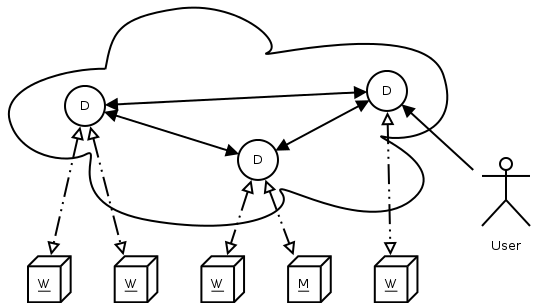
\includegraphics[height=4in]{imageinput/grob-layout-komponenten.png}
  \end{center}
  \caption{Grundlegende Datenstrukturen}
\end{figure}




\subsection{Grundlegendes Datenmodell}


\begin{figure}[ht] 
  \label{fig:datenstrukturen}
  \begin{center}
      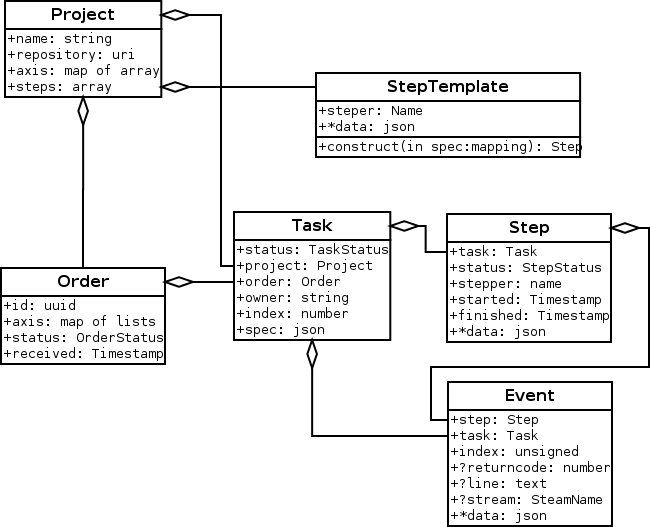
\includegraphics[height=4in]{imageinput/datenstrukturen-step-templates.png}
  \end{center}
  \caption{Grundlegende Datenstrukturen}
\end{figure}




\section{Vorbereitende Primitiven}
\subsection{watch\_for}
\subsection{run\_callbacks}

\section{Projektkonfiguration}

\section{Auftragsannahme}

\begin{figure}[ht] 
  \label{fig:lebenszyklus-auftrag-eingang}
  \begin{center}
      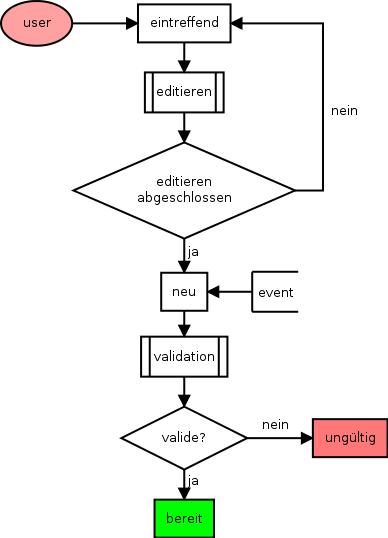
\includegraphics[height=5in]{imageinput/lebenszyklus-auftrag-eingang.png}
  \end{center}
  \caption{Auftragsannahme: Flowgraph}
\end{figure}


\subsection{Eingang}
\subsection{Validation}

\section{Management}



\begin{figure}[ht] 
  \label{fig:lebenszyklus-auftrag-abarbeitung}
  \begin{center}
      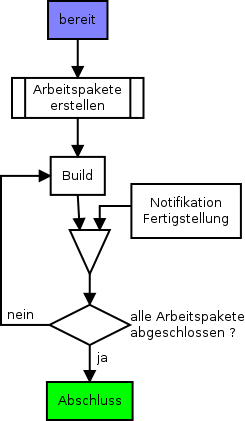
\includegraphics[height=4in]{imageinput/lebenszyklus-auftrag-abarbeitung.png}
  \end{center}
  \caption{Auftragsannahme: Flowgraph}
\end{figure}

\subsection{Auftragsvorbereitung}
\subsection{Bereitstellung von Arbeitspacketen}
\subsection{Abschluss von auftr\"agen}


\section{Zuteilung/Abarbeitung von Arbeitspacketen}
\subsection{Zuteilungsmethoden}

\subsubsection{\"Uberblick}

\begin{verbatim}

- methoden
    - token basiert
    - ausschreibungsbasiert

\end{verbatim}


\subsubsection{token basierte zuweisung}

\begin{verbatim}
- arbeiter teilen nur mit, dass sie arbeitsfaehig sind
- manager kontrolliert wer welchen auftrag erhaelt
- fuer erweiterte use-cases extra wissen im manager notwendig
\end{verbatim}

\begin{figure}[ht] 
  \label{fig:auftrag-zuteilung-token}
  \begin{sequencediagram}
      \newinst{worker}{:Worker}
      \newinst[1]{manager}{:Manager}
      \mess{worker}{token <spec>}{manager}
      \mess{manager}{work <spec>}{worker}
      \mess{worker}{result}{manager}
  \end{sequencediagram}
  \caption{Auftragszuteilung: Tokenbasiert}
\end{figure}

\subsubsection{ausschreibungsbasierte zuweisung}

\begin{verbatim}
- manager teilt offene auftraegeposten mit (in datenbank verf.)
- arbeiter konkurieren um offene auftraege
- manager entscheidet wer den aufrag dann erhaelt


- autonomere arbeiter
- manager muss nur noch entscheiden wer, nicht mehr warum
- aufgrund der datenbank konzeptuell einfacher
\end{verbatim}

\begin{figure}[ht] 
  \label{fig:auftrag-zuteilung-claim}
  \begin{sequencediagram}
      \newinst{workera}{:Worker A}
      \newinst[1]{manager}{:Manager}
      \newinst[1]{workerb}{:Worker B}
      \mess[1]{manager}{availiable}{workera}
      \prelevel
      \prelevel
      \mess[1]{manager}{availiable}{workerb}

      \mess[1]{workera}{claim}{manager}
      \prelevel
      \prelevel
      \mess[2]{workerb}{claim}{manager}
      %XXX: better call?
      %\prelevel
      %\prelevel
      %\begin{call}{manager}{approve}{manager}{workera}
      %\end{call}
      \mess{manager}{approve A}{workera}
      \prelevel
      \mess{manager}{approve A}{workerb}
  \end{sequencediagram}
  \caption{Auftragszuteilung: Ausschreibungsbasiert}
\end{figure}


\subsection{Vorbereitung Abarbeitung}
\subsection{Abschluss Abarbeitung}


\section{Abarbeitung von Arbeitspacketen}
\subsection{Arbeitsschritte}
\begin{figure}[ht] 
  \label{fig:lebenszyklus-arbeitsschritt}
  \begin{center}
      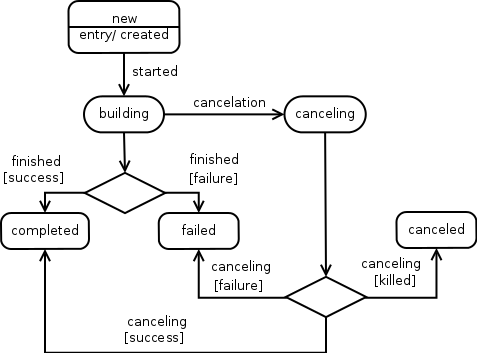
\includegraphics[height=3.4in]{imageinput/lebenszyklus-arbeitsschritt.png}
  \end{center}
  \caption{Stategraph eines Arbeitschrittes}
\end{figure}

\begin{verbatim}
- kill wird in der impl nicht betrachtet
\end{verbatim}


\subsection{Datensammlung zur Laufzeit}
\subsection{Datensammling nach Abschluss eines Schrittes}
\subsection{Abschluss von Arbeitschritten}


\section{Arten von Arbeitschritten}
\subsection{Prozessaktionen}
\subsection{Quellcode Management Aktionen}
\subsection{Theoretische Betrachtung Interaktion}
